\subsection{State of the Art}

\begin{frame}[t]{Echo-aware Applications \hfill\faBook}

    \begin{block}{Echoes: same content, different time/direction}
        \centering
        \only<1>{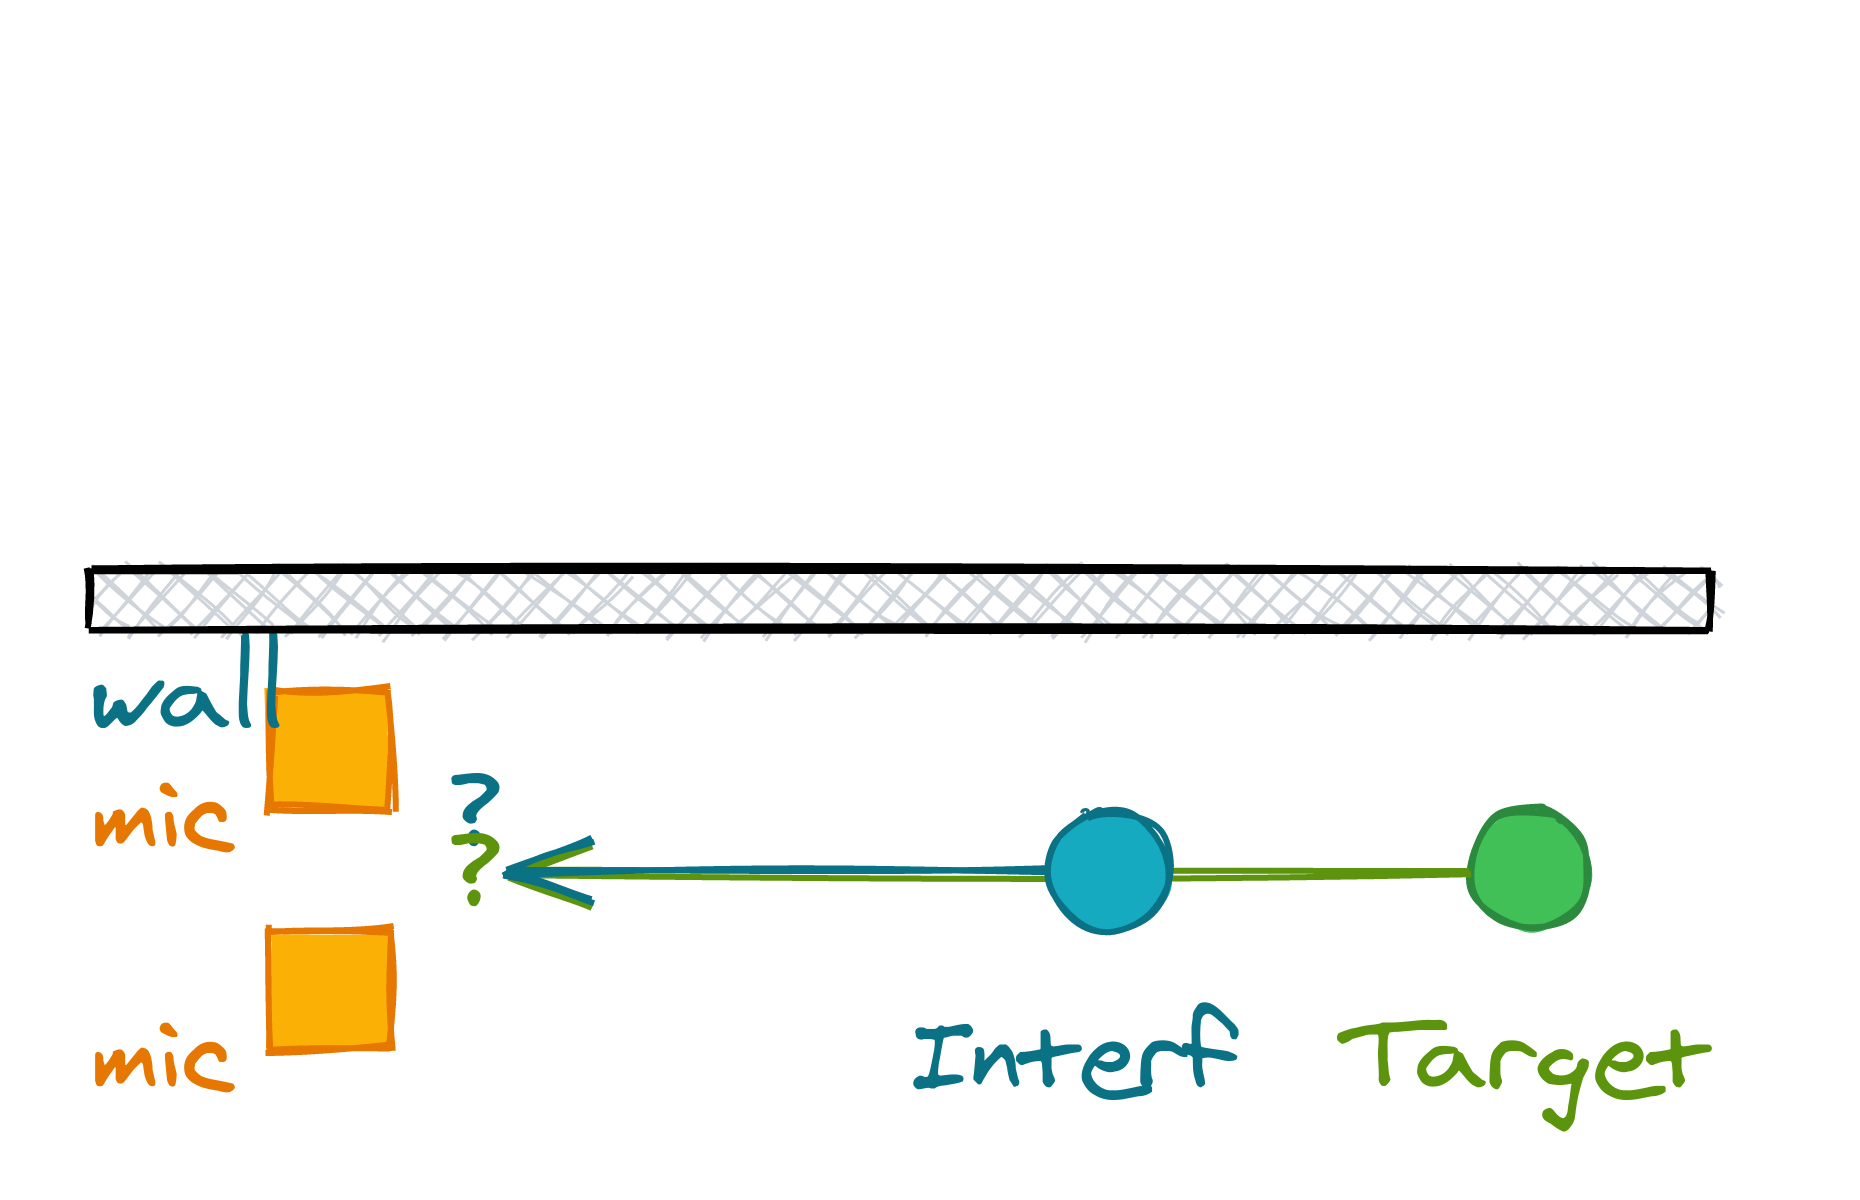
\includegraphics[width=0.45\textwidth]{figures/image_src_mic(0).png}}%
        \only<2>{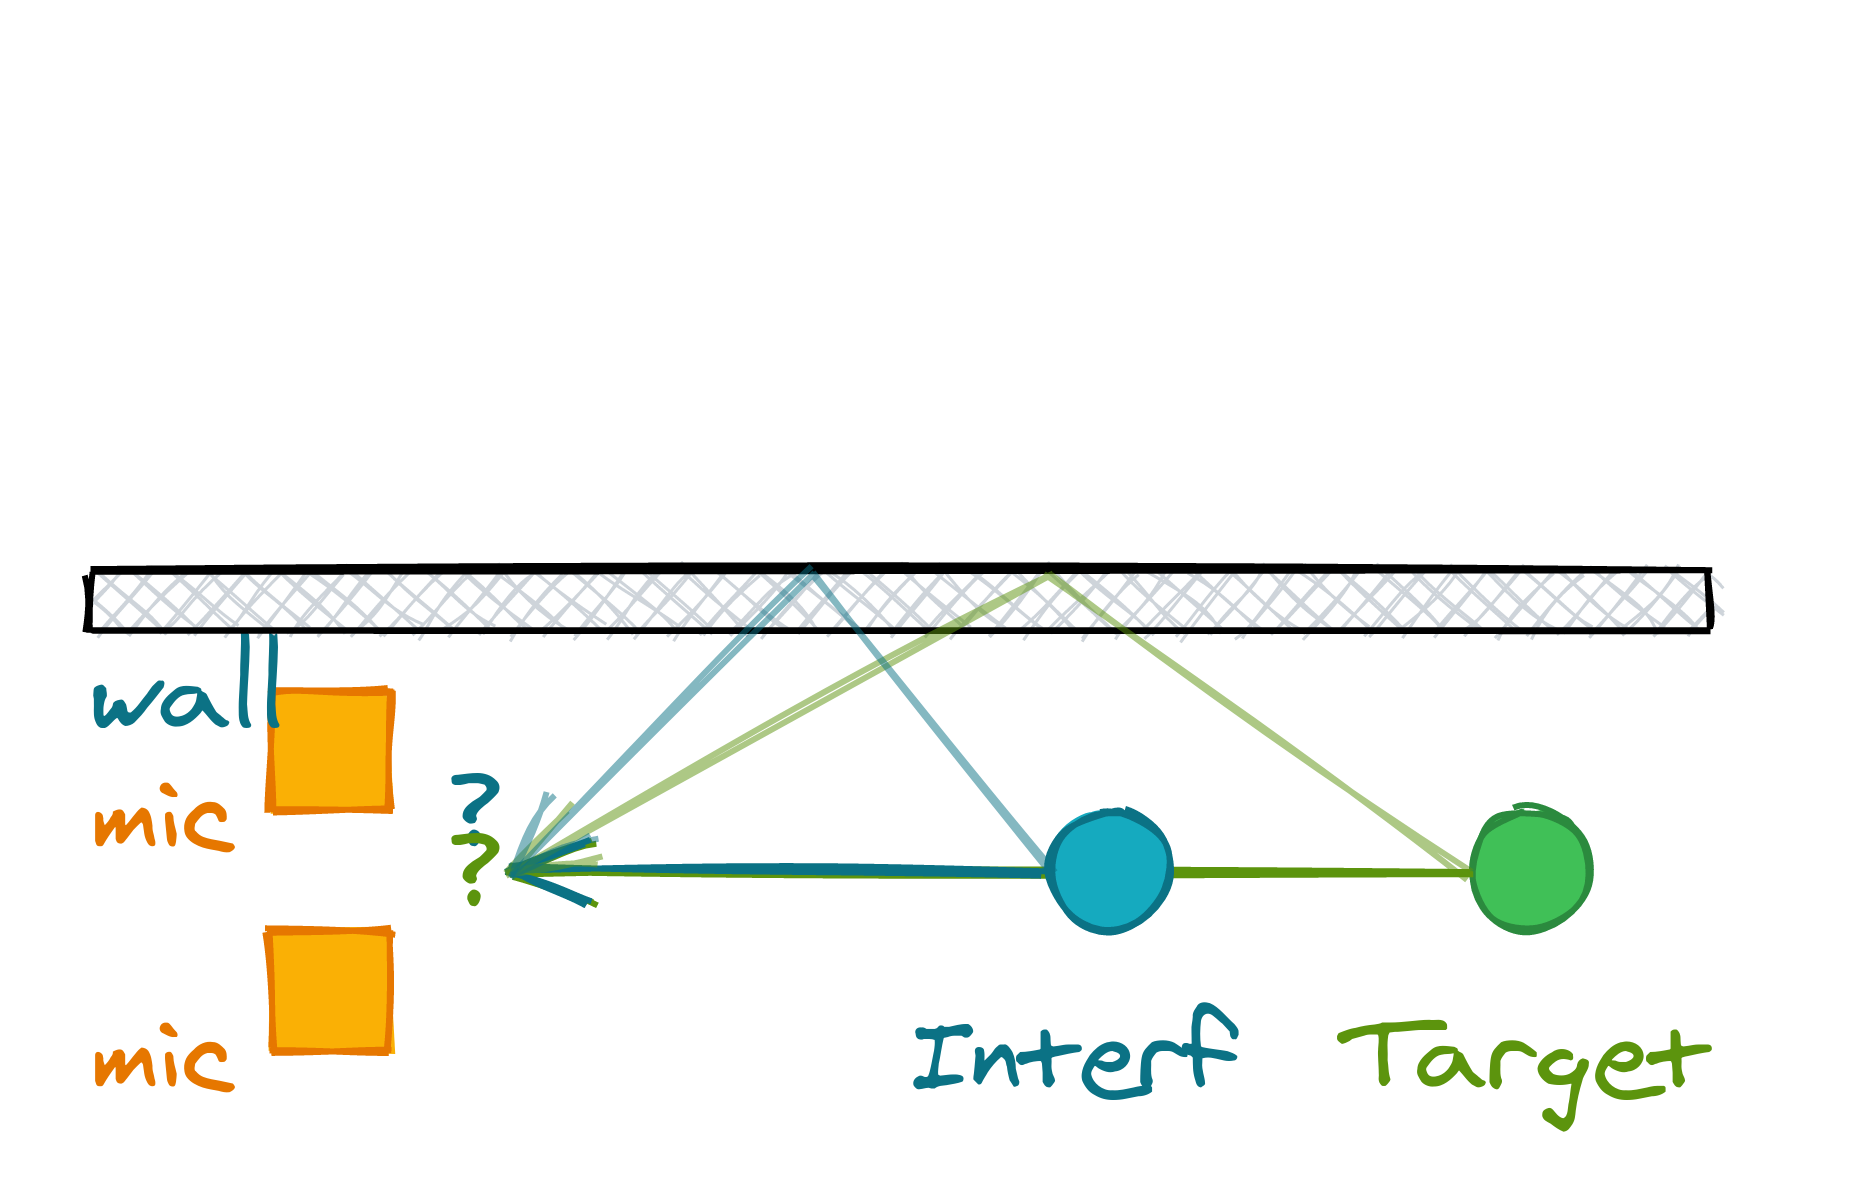
\includegraphics[width=0.45\textwidth]{figures/image_src_mic(1).png}}%
        \only<3>{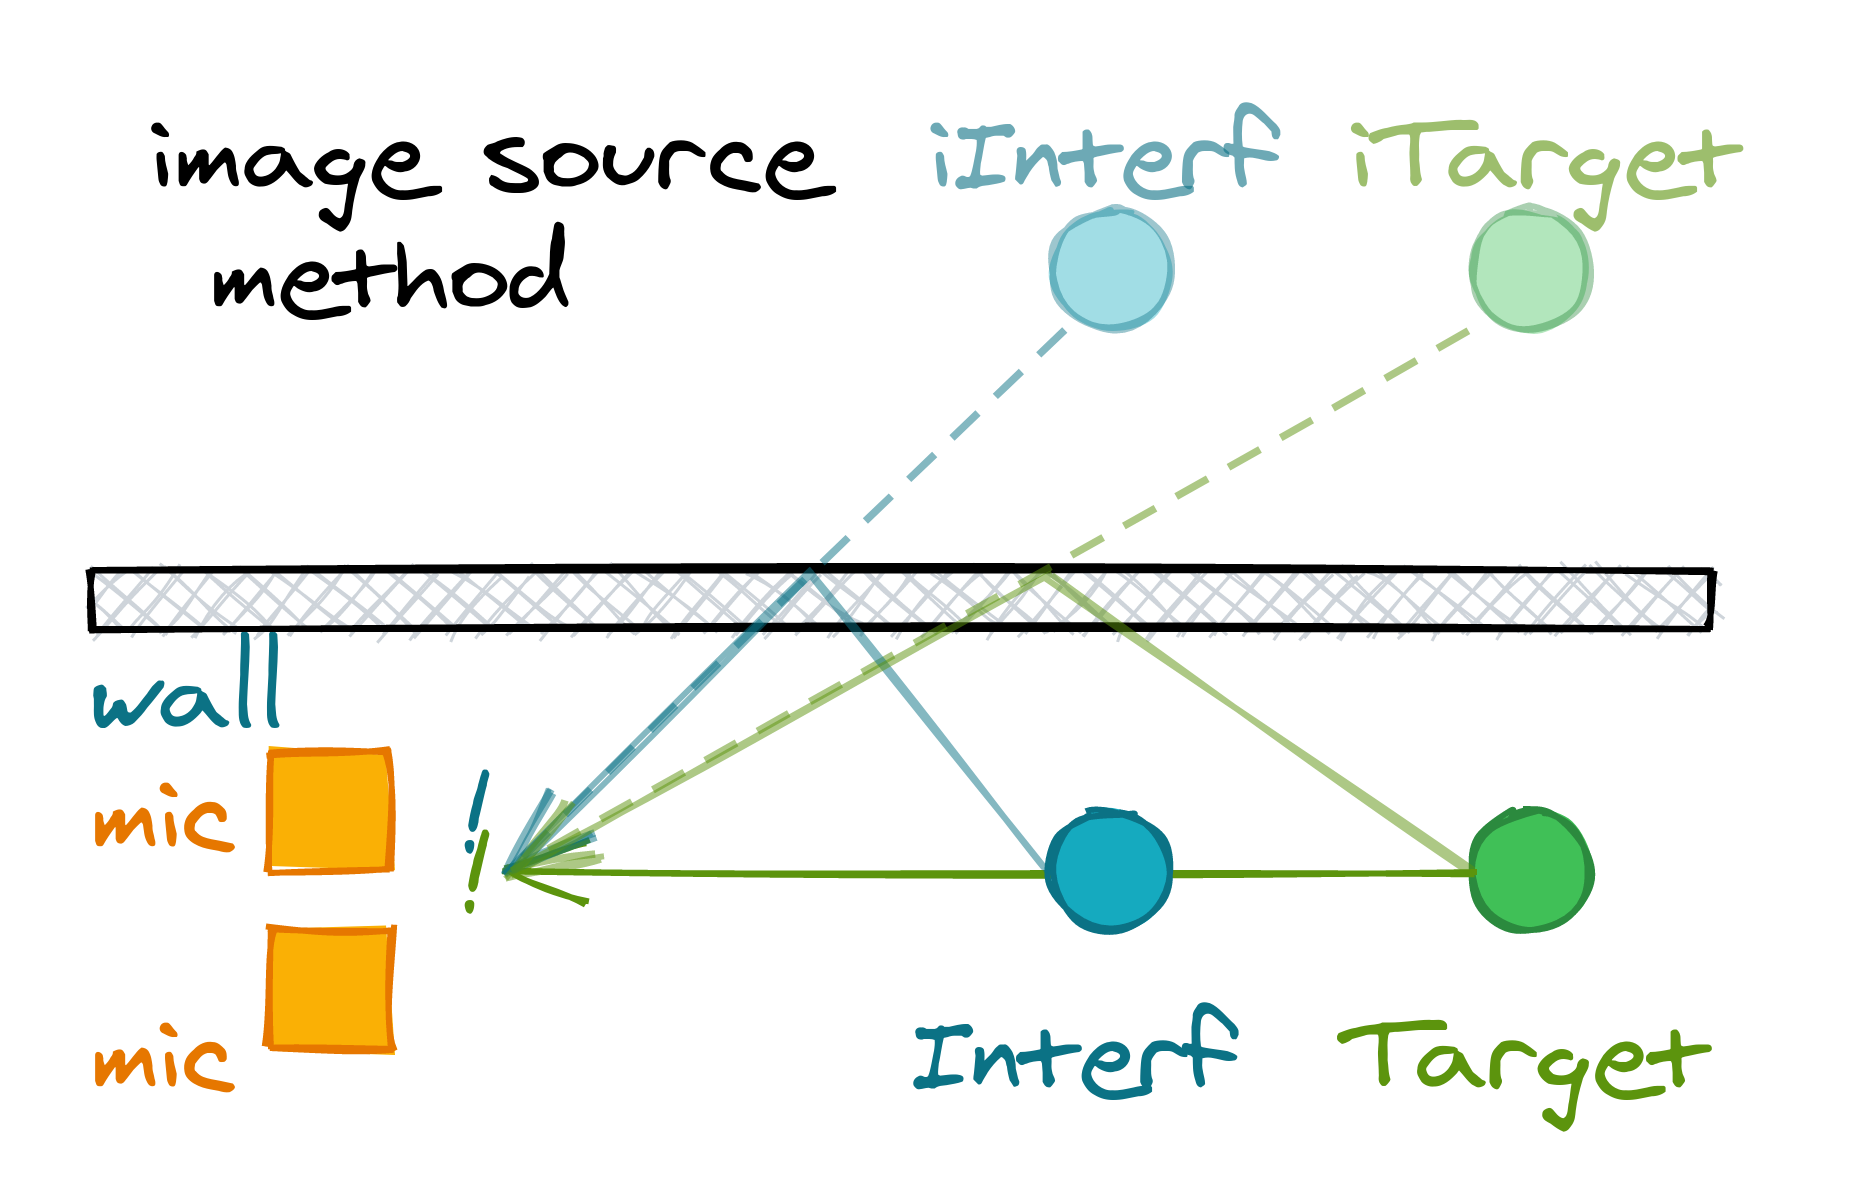
\includegraphics[width=0.45\textwidth]{figures/image_src_mic(2).png}}%
        \only<4->{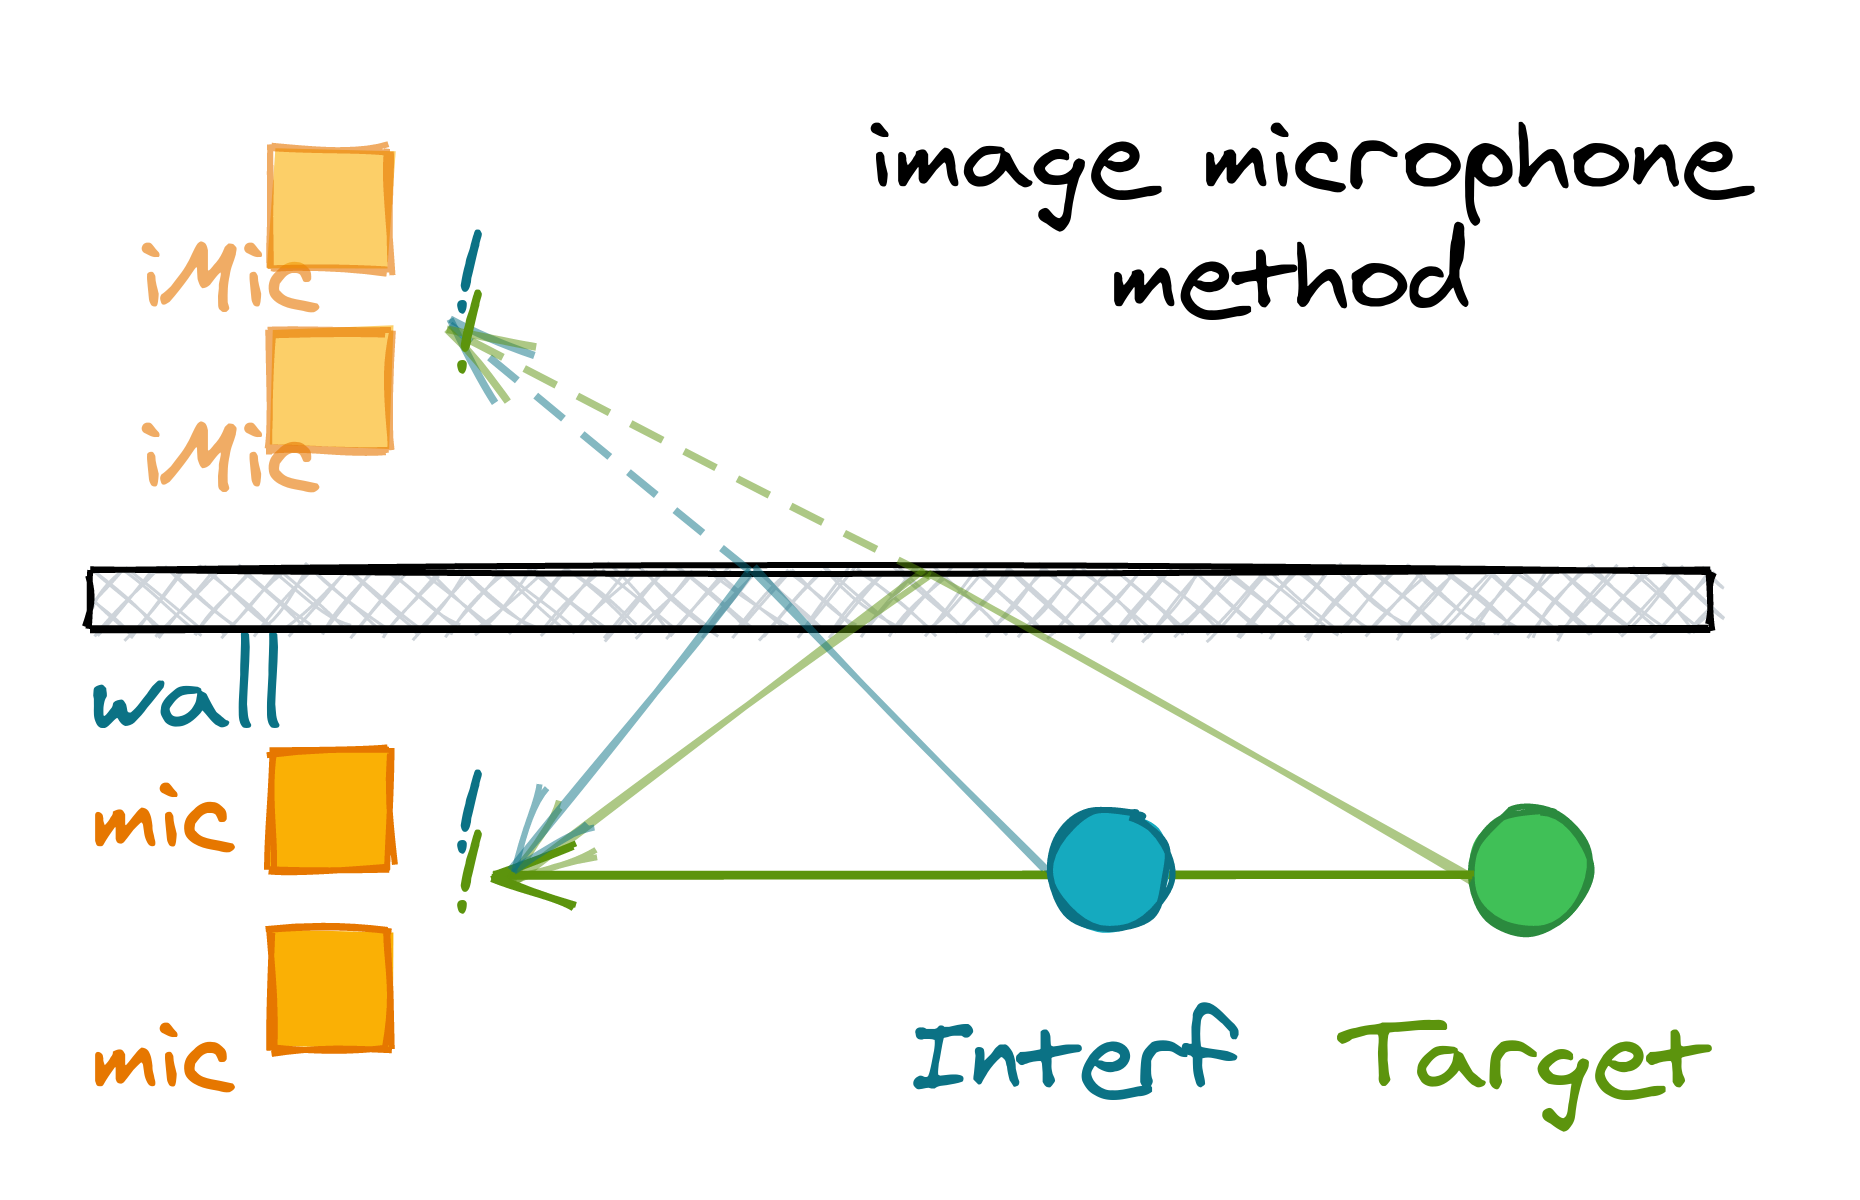
\includegraphics[width=0.45\textwidth]{figures/image_src_mic(3).png}}%
    \end{block}

    \pause[4]
    \begin{textblock*}{30mm}(95mm,35mm)
        \centering
        \small
        \visible<4->{
        \textcolor{myred}{%
            Image Source Model
            \\$\Leftrightarrow$
            \\Image Microphone Model}}
    \end{textblock*}

    \pause[5]
    \begin{columns}[T,onlytextwidth]
        \column{.32\textwidth}
        \begin{block}{\textbf{What?}}
            \small
            Echoes = copy

            \vspace{-2mm}
            \begin{itemize}
                \item \only<-7>{Sound Source Separation}\only<8>{\alert{Sound Source Separation}}\only<9->{\textcolor{gray}{Sound Source Separation}}
                \\{\footnotesize\cite{leglaive2016multichannel}}
                \item \only<-7>{Speech Enhancement}\only<8->{\alert{Speech Enhancement}}
                \\{\footnotesize\cite{flanagan1993spatially,dokmanic2015raking,kowalczyk2019raking}}
            \end{itemize}
        \end{block}
        \column{.32\textwidth}
        \pause[6]
        \begin{block}{\textbf{Where?}}
            \small
            Echoes $\gets$ image

            \vspace{-2mm}
            \begin{itemize}
                \item \only<-7>{Sound Source Localization}\only<8->{\alert{Sound Source Localization}}
                \\{\footnotesize\cite{ribeiro2010turning,jensen2019method}}
                \item \only<-7>{Room Geometry Estimation}\only<8>{\alert{Room Geometry Estimation}}\only<9->{\textcolor{gray}{Room Geometry Estimation}}
                \\{\footnotesize\cite{antonacci2012inference,crocco2017uncalibrated}}
            \end{itemize}
        \end{block}
        \column{.32\textwidth}
        \pause[7]
        \begin{block}{\textbf{How?}}
            \small
            Echoes $\in$ sound propagation

            \vspace{-2mm}
            \begin{itemize}
                \item Blind Channel Estimation
                \\{\footnotesize\cite{lin2007blind,crocco2017uncalibrated}}
                \item Acoustic Measurements
                \\{\footnotesize\cite{eaton2015ace,kuttruff2016room}}
            \end{itemize}
        \end{block}
    \end{columns}

    \pause[5]
    \vspace{-3mm}
    \begin{center}
        \textcolor{gray}{\small (In-depth literature review in \faBook.)}
    \end{center}
\end{frame}

\begin{frame}{Sound Source Localization (SSL) {\hfill\small (common knowledge)} \faBook}

    \faAlert We do not consider here distance estimation.

    \begin{columns}[T,onlytextwidth]
        \column{0.6\textwidth}
        \begin{block}{SSL with 2 microphones}
            \begin{itemize}
                \item Only one angle of arrival (\alert{AOA})\iconAOA
                \item Can be approximated from \alert{TDOA} using e.g. \GCCPHAT\footnotemark[1]
                \\\addendum{known limitation, but good in practice}\footnotemark[2]
            \end{itemize}
        \end{block}
        \column{0.38\textwidth}
        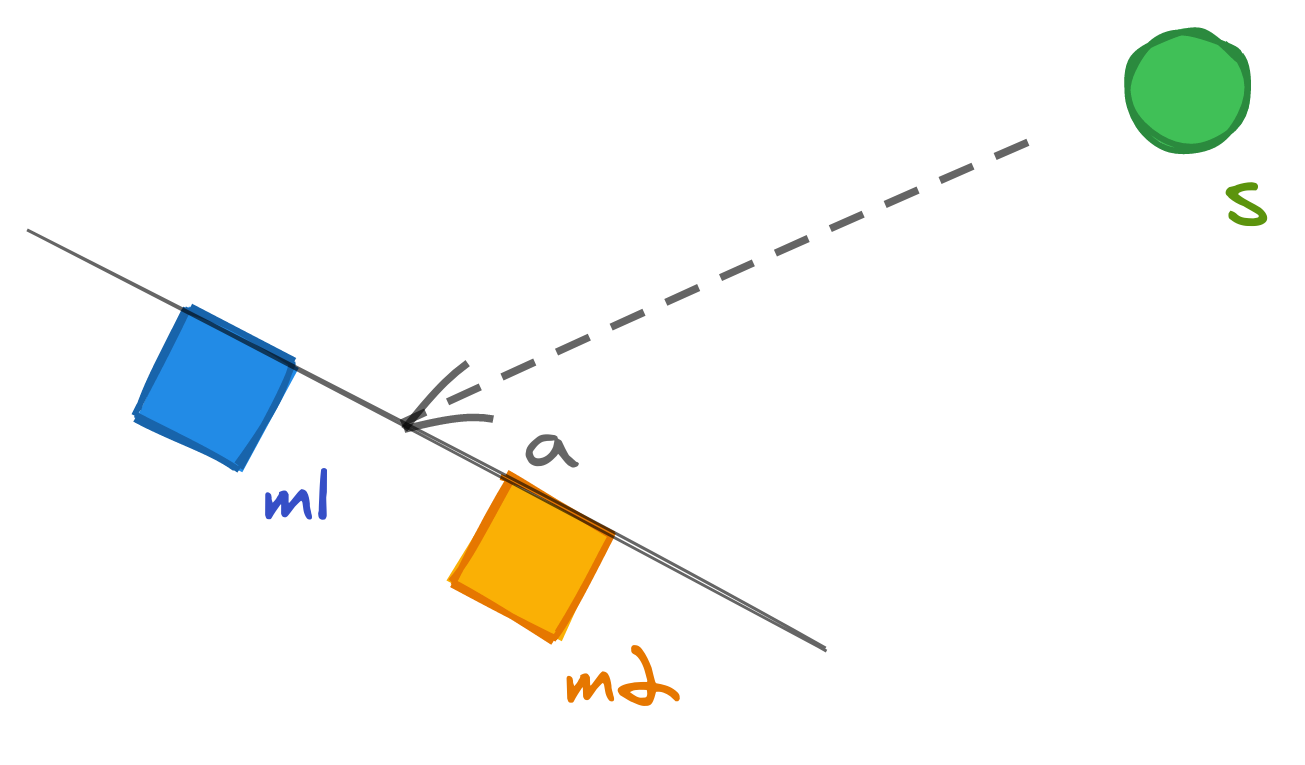
\includegraphics[width=\textwidth]{figures/1d_ssl.png}
    \end{columns}
    \pause

    \begin{columns}[T,onlytextwidth]
        \column{0.6\textwidth}
        \begin{block}{SSL with more microphones}
            \begin{itemize}
                \item Two Direction of Arrival (DoA):
                \\azimuth (\faArrowsAltH) and elevation (\faArrowsAltV)
                \item AOA at each pair can be ``fused'' together
                \\\addendum{e.g., angular spectra in SRP-PHAT\footnotemark[2]}
                \\\addendum{known limitation, but good in practice}\footnotemark[3]
            \end{itemize}
        \end{block}
        \column{0.38\textwidth}
        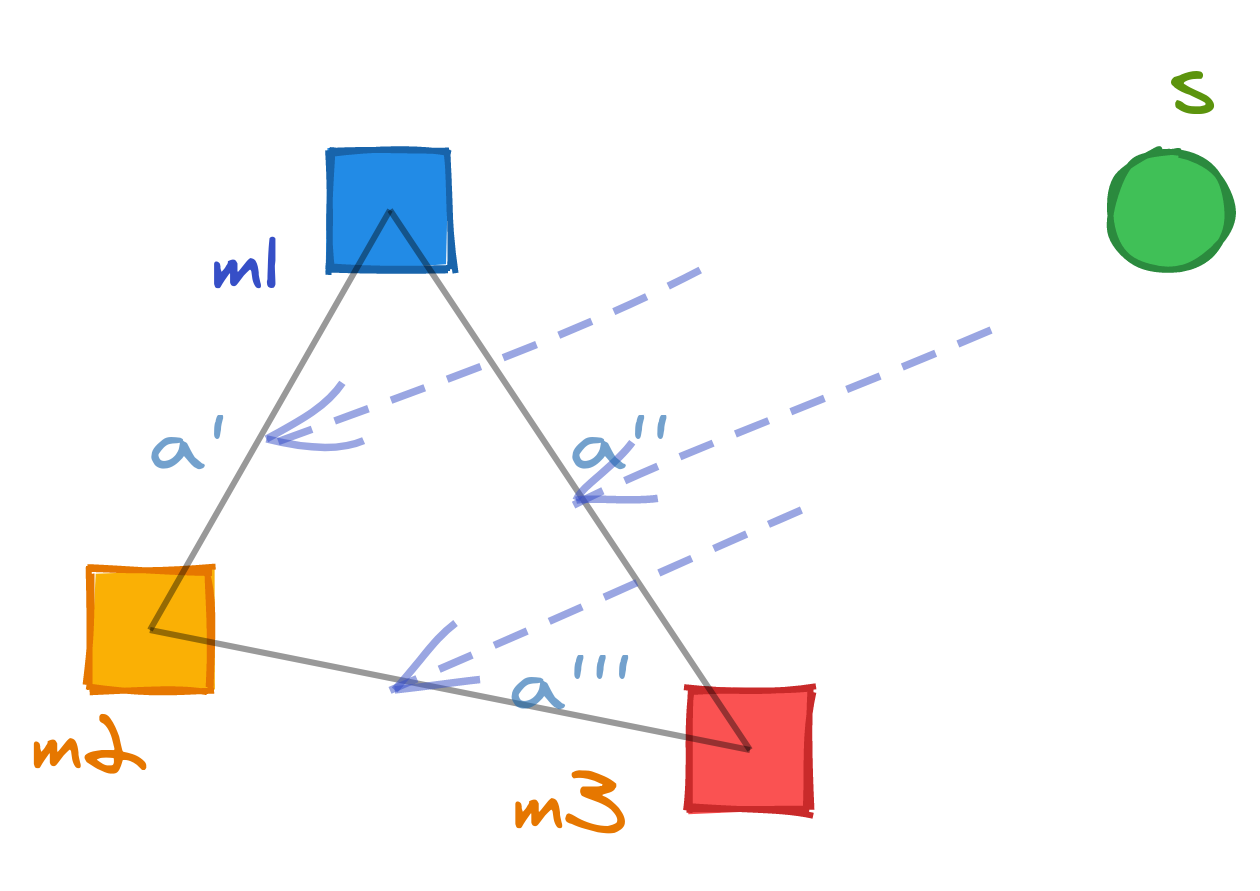
\includegraphics[width=\textwidth]{figures/2d_ssl.png}
    \end{columns}

    \footnotetext[1]{\tiny~\cite{knapp1976generalized}}
    \footnotetext[2]{\tiny~\cite{dibiase2001robust}}
    \footnotetext[3]{\tiny~\cite{lebarbenchon2018evaluation}}

\end{frame}

\subsection{Echo-aware Sound Source Localization}

\begin{frame}[t]{Sound Source Localization \alert{with Echoes} \hfill\faMapMarked*}

    \vspace*{2mm}
    \begin{columns}[T,onlytextwidth]

        \begin{column}{0.5\textwidth}
            \begin{block}{The \alert{Picnic} Scenario:}
                \begin{itemize}
                    \small
                    \item<1-> One source
                    \item<1-> Two microphones
                    \begin{itemize}
                        \item<1->[$\rightarrow$] passive scenario
                        \item<1->[$\rightarrow$] generalizable to any array geometry
                    \end{itemize}
                    \item<2-> Close to a very reflective surface
                    \begin{itemize}
                        \item<2->[$\rightarrow$] First echo = Strongest echo
                        \item<2->[$\rightarrow$] $\alpha_\text{picnic}$ const. $\forall f$
                        \item<2->[$\rightarrow$] table-top device
                    \end{itemize}
                \end{itemize}
            \end{block}
        \end{column}

        \begin{column}{0.5\textwidth}
            \centering
            \only<1,2>{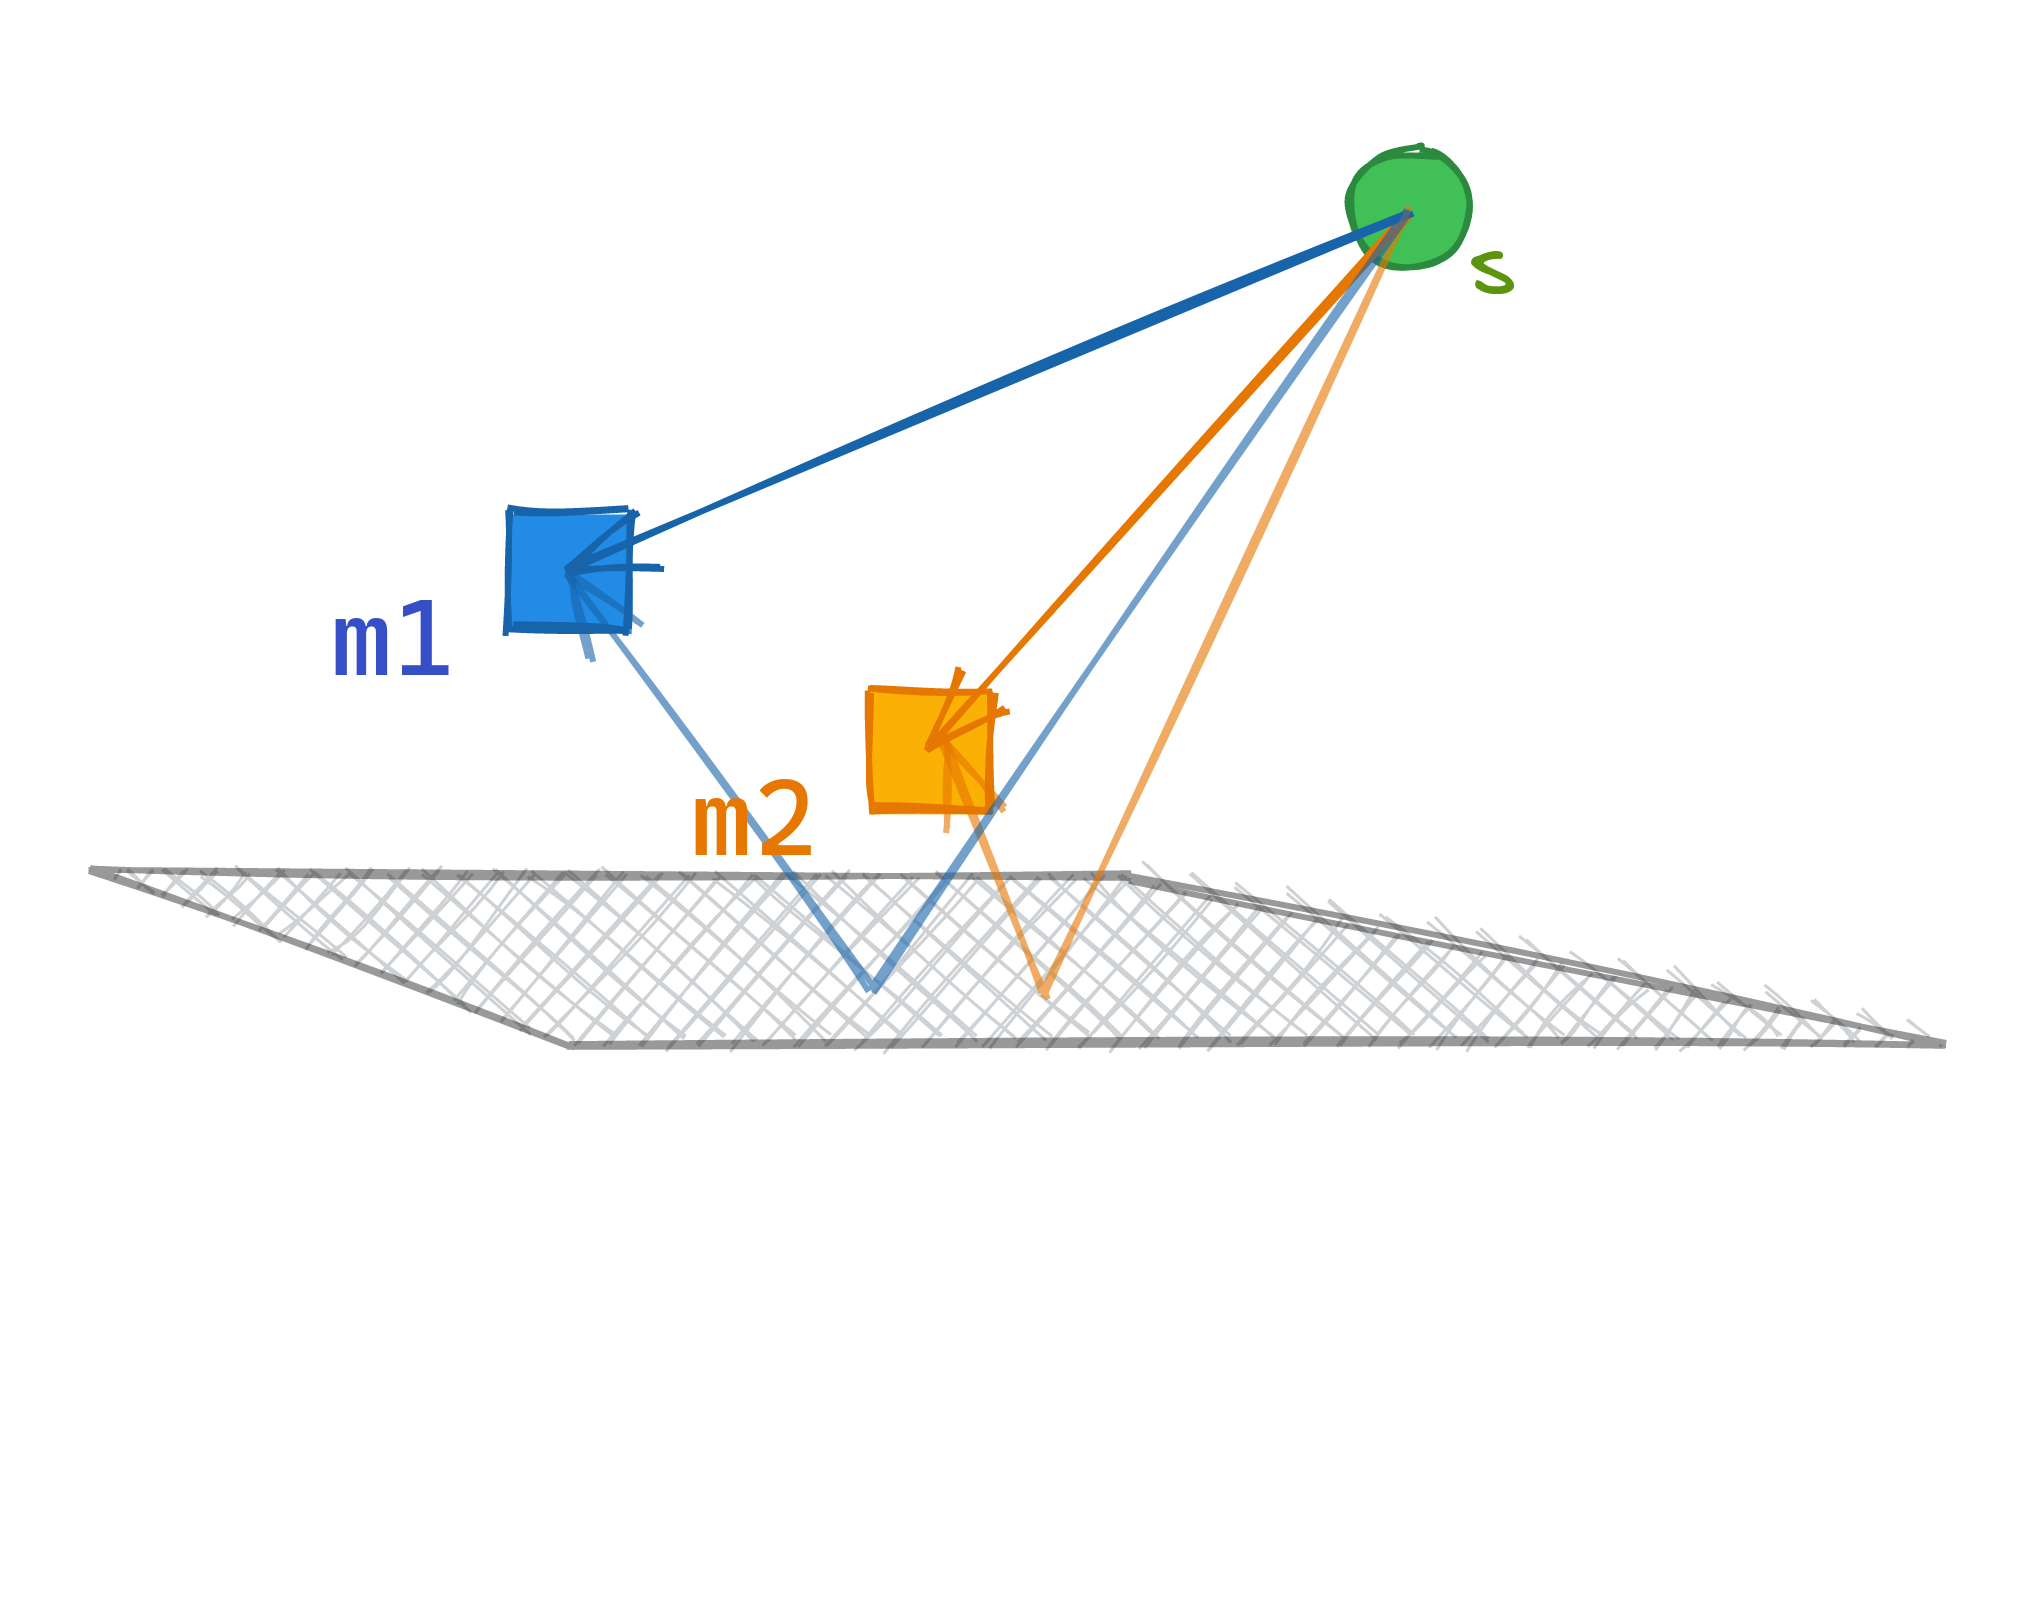
\includegraphics[width=0.9\textwidth]{figures/mirage1.png}}%
            \only<3,4>{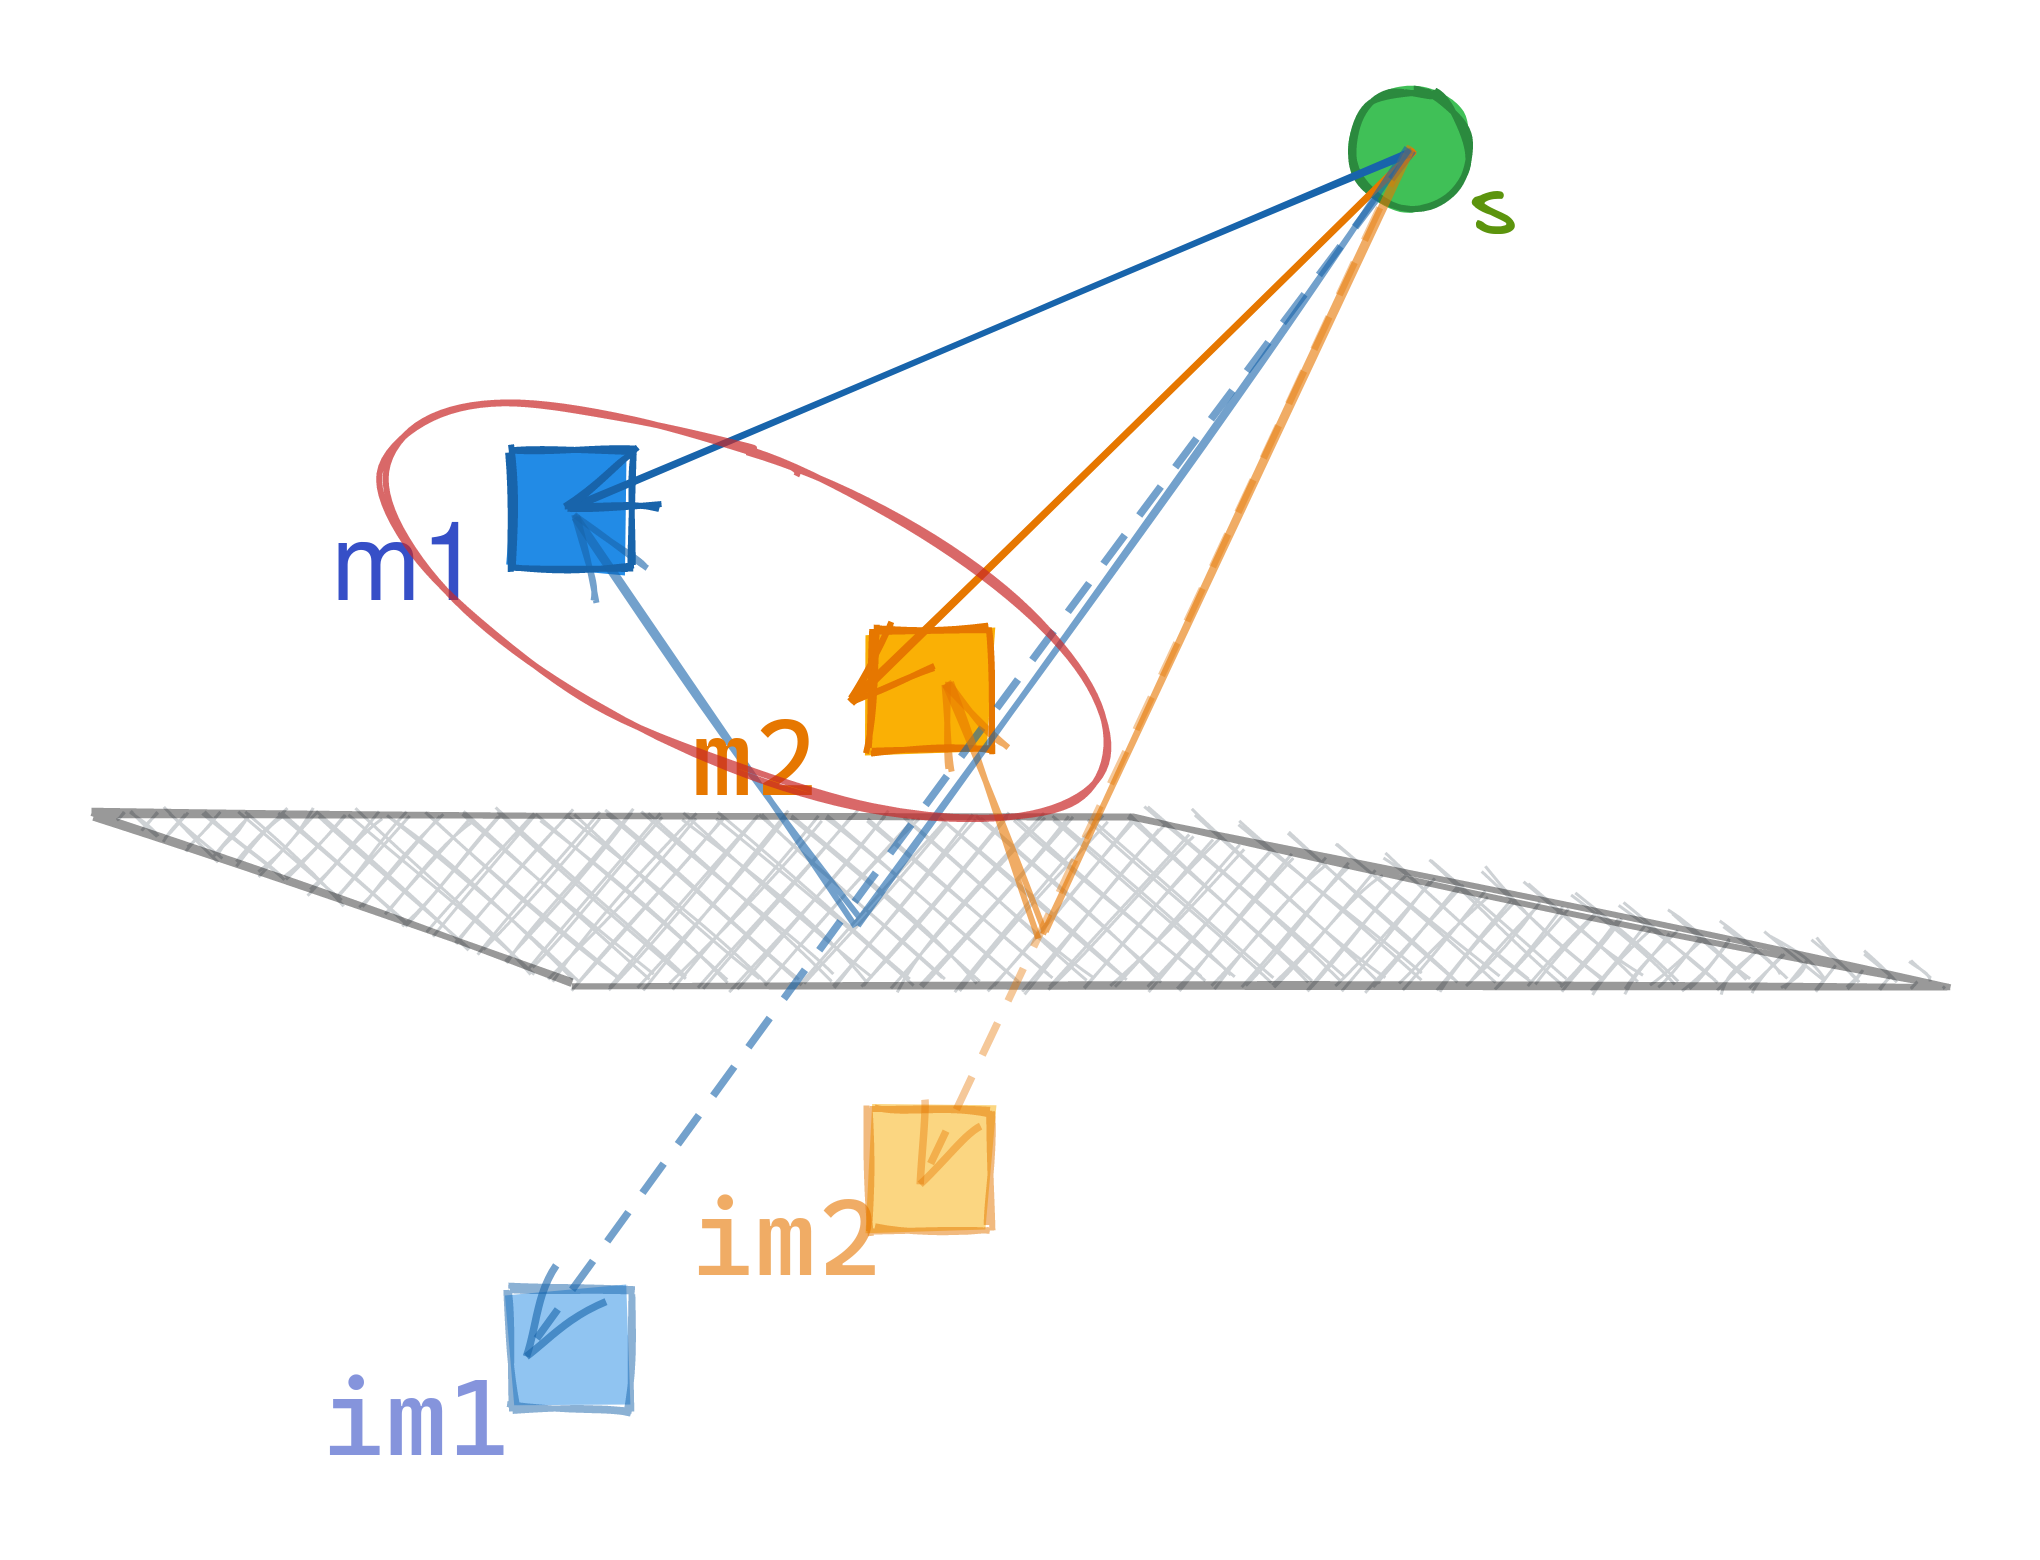
\includegraphics[width=0.9\textwidth]{figures/mirage2.png}}%
            \only<5>{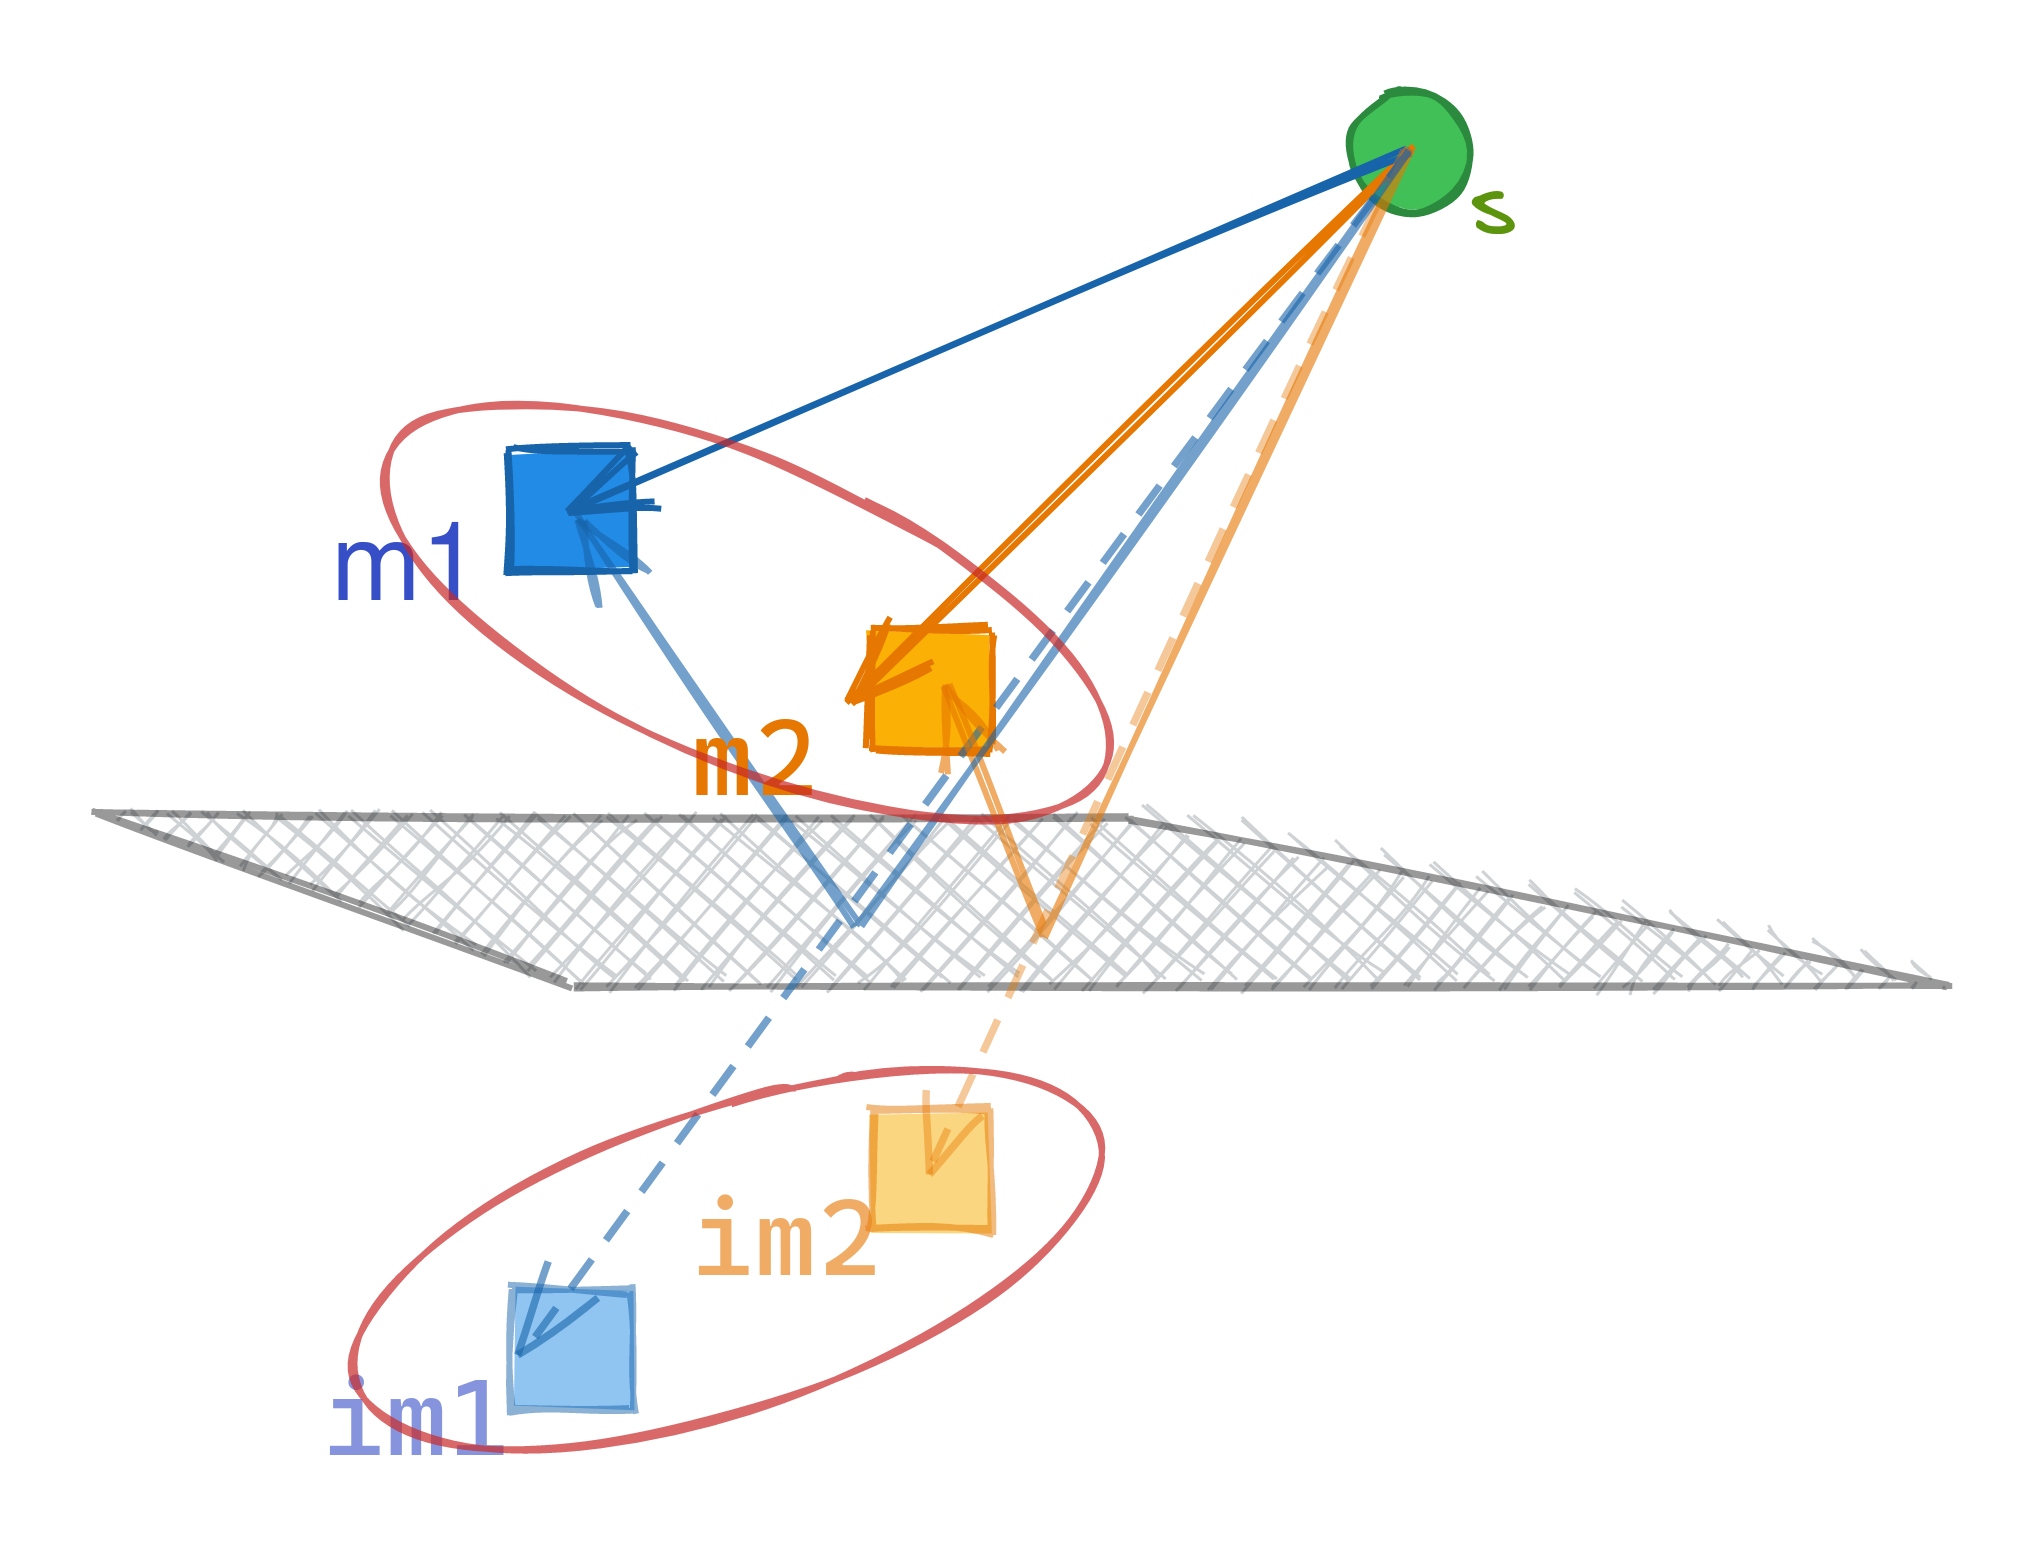
\includegraphics[width=0.9\textwidth]{figures/mirage3.png}}%
            \only<6>{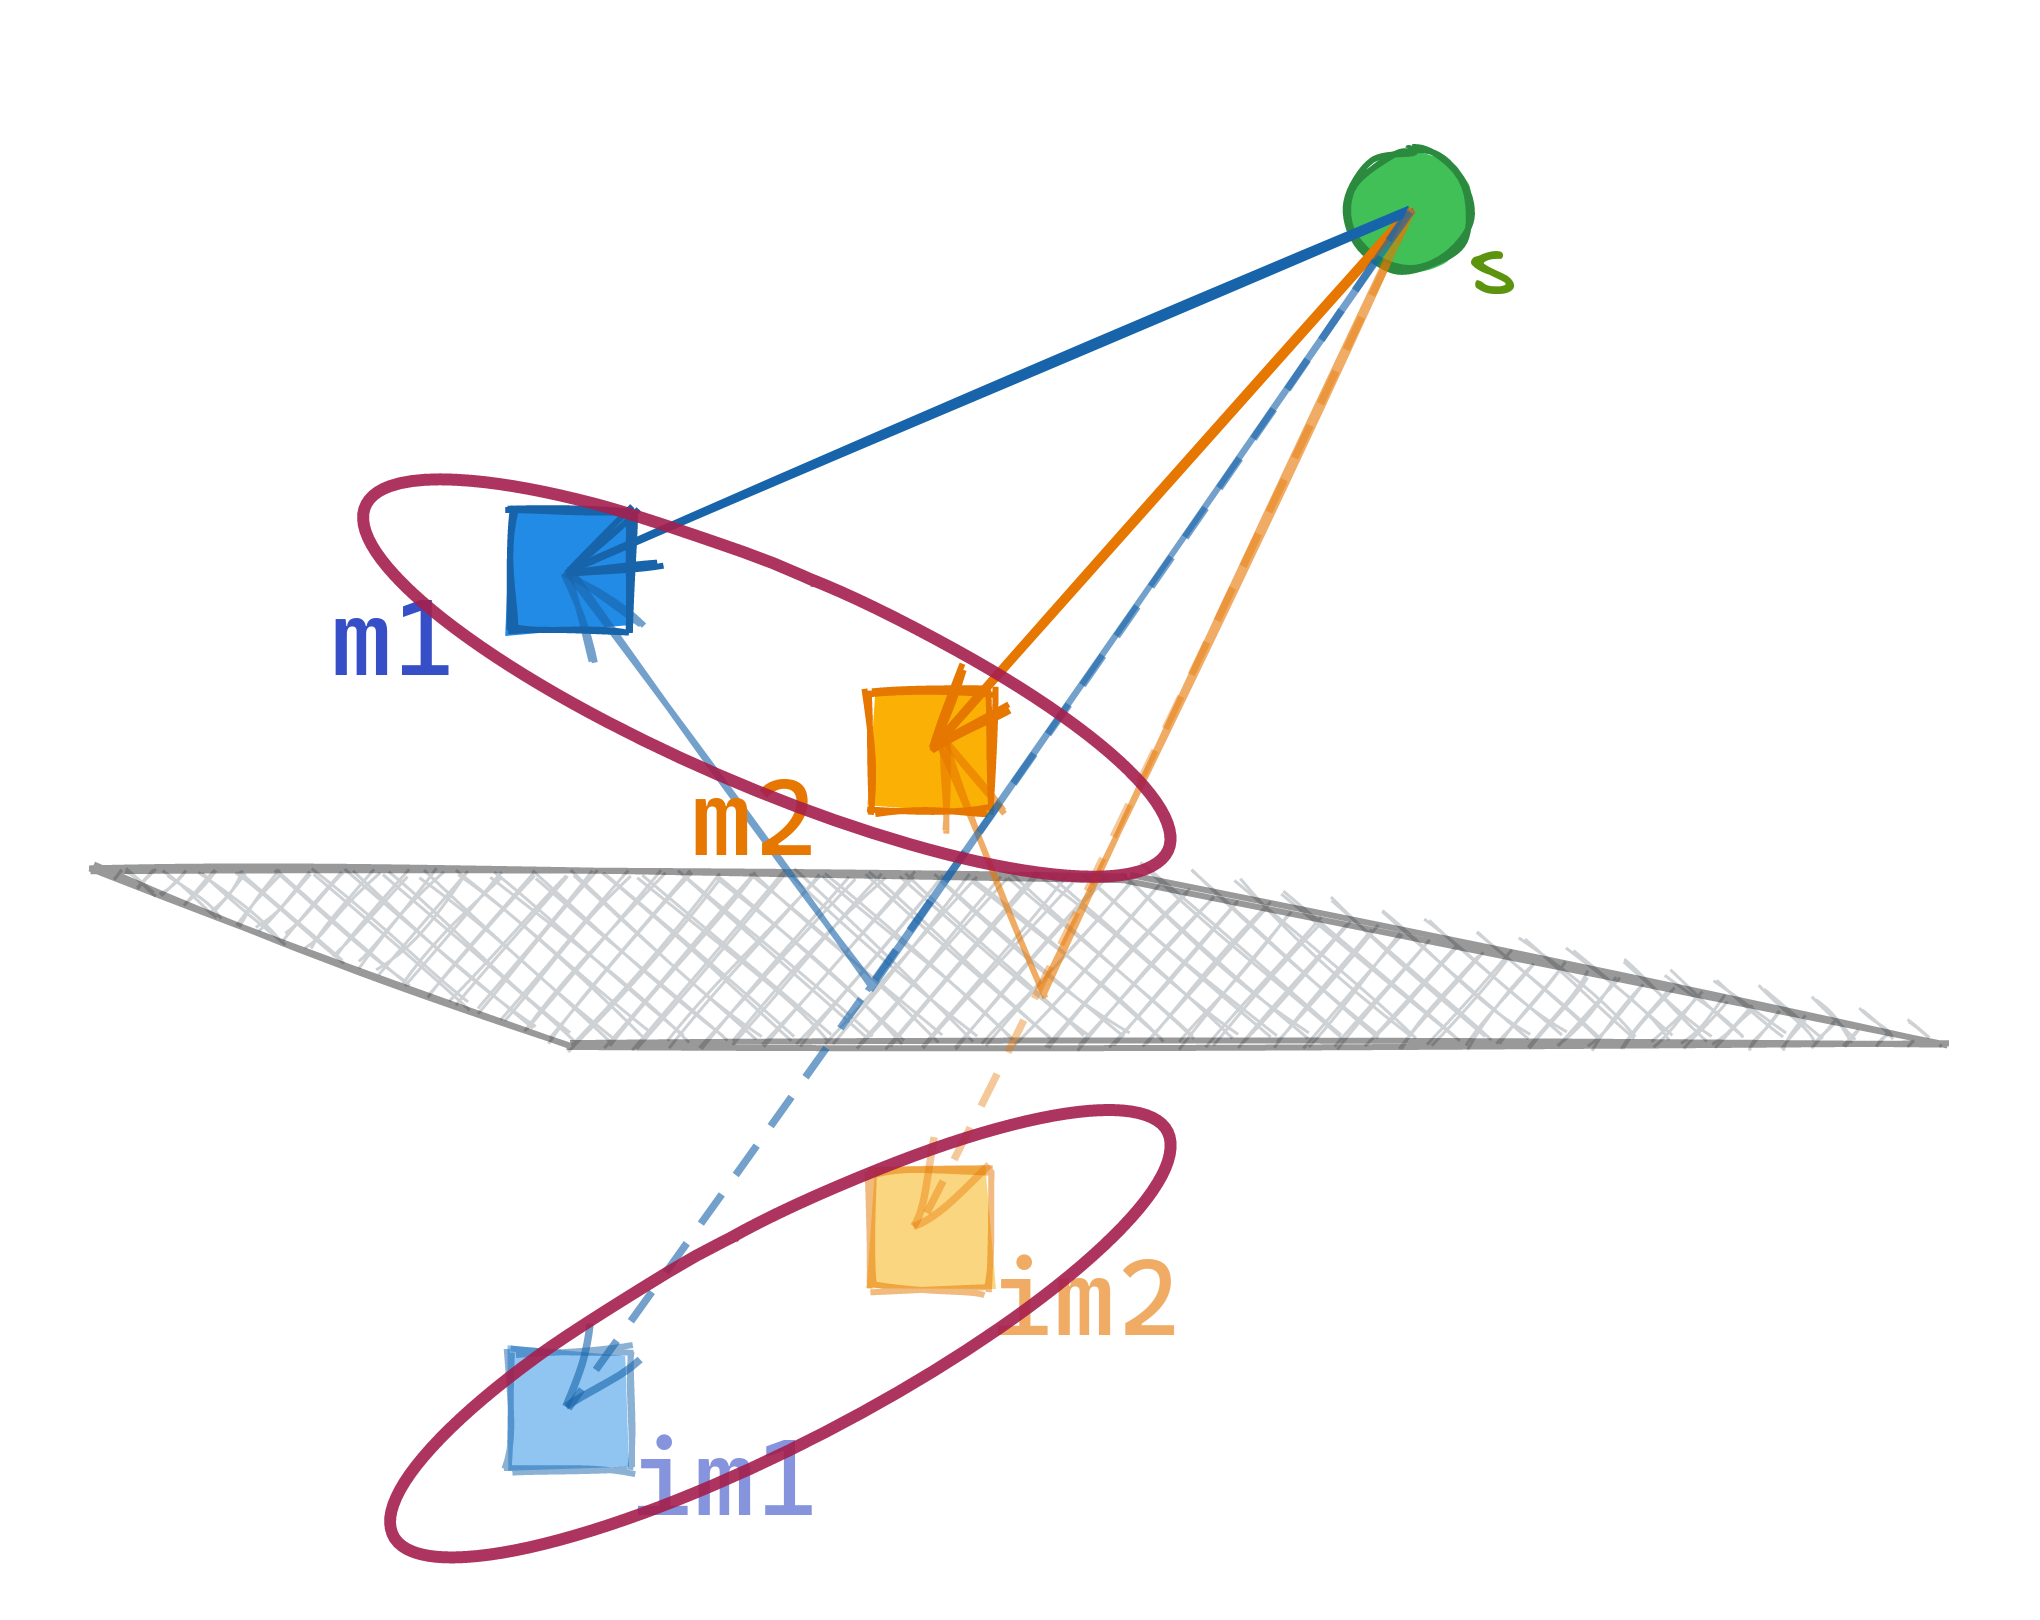
\includegraphics[width=0.9\textwidth]{figures/mirage4.png}}%
            \only<7>{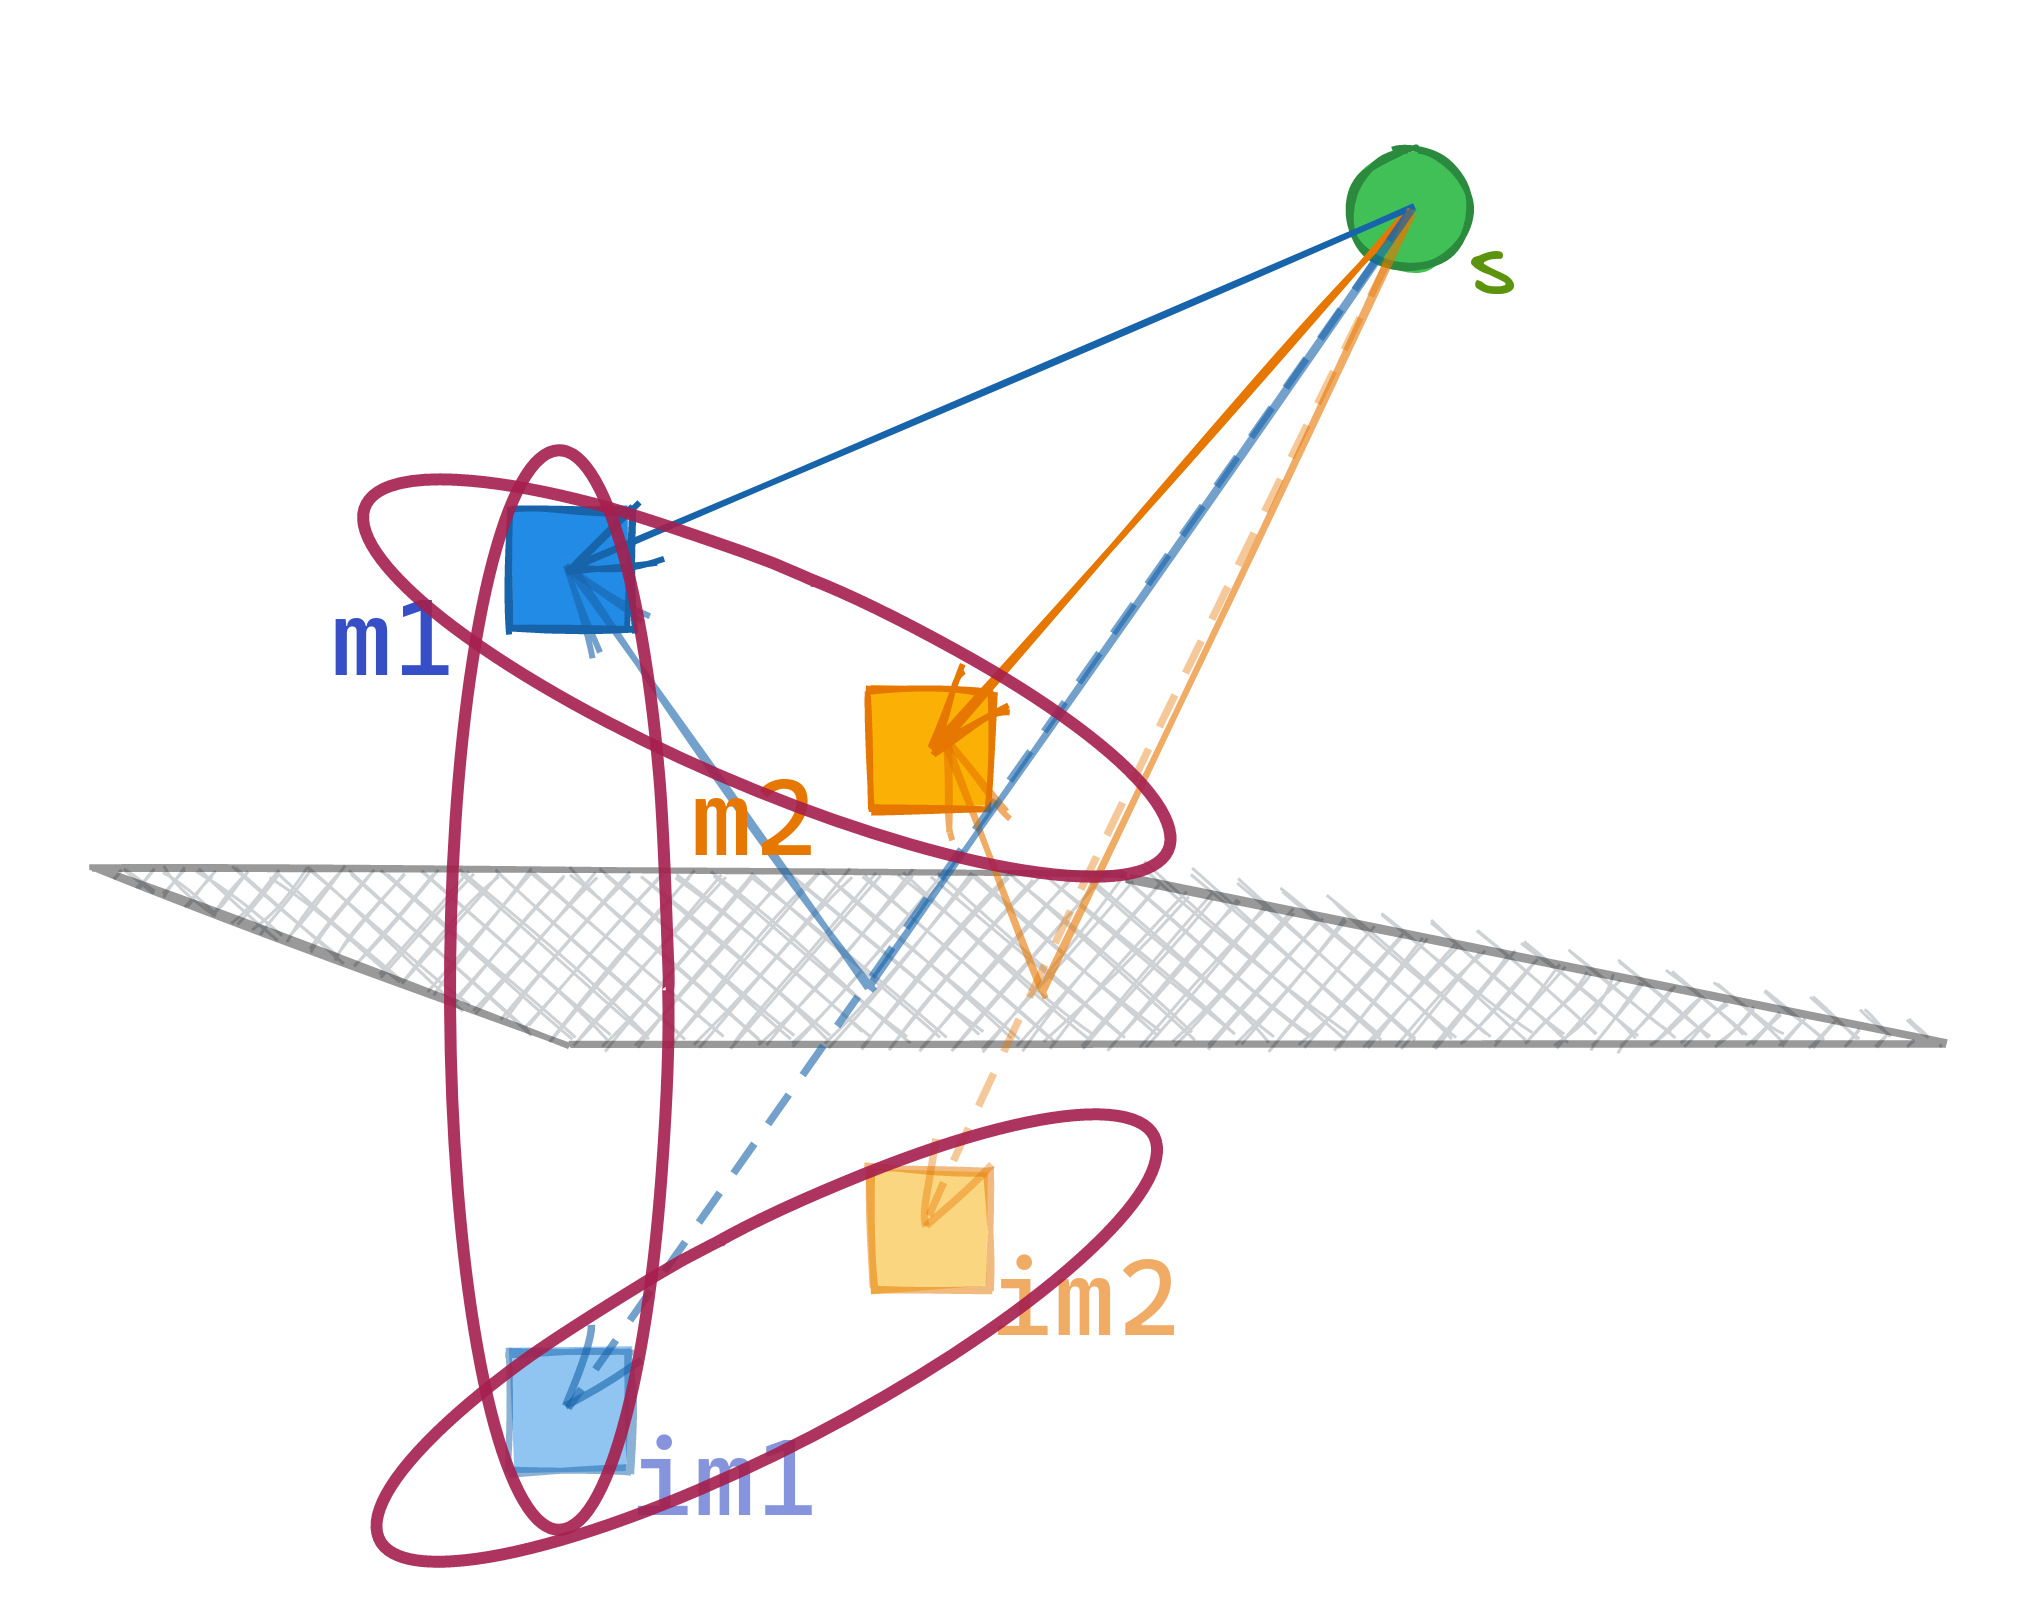
\includegraphics[width=0.9\textwidth]{figures/mirage5.png}}%
        \end{column}
    \end{columns}

    \pause[3]
    \vfill
    \begin{columns}[T,onlytextwidth]

        \begin{column}{0.5\textwidth}
            \begin{block}{Each pair is augmented with echoes}
                \begin{center}
                    \textcolor{myred}{\textbf{Mirage Array}}
                    \\\addendum{Microphone Array Augmetation with Echoes}
                \end{center}
            How to access the \textit{image} microphones?
            \end{block}
        \end{column}

        \visible<4->{
        \begin{column}{0.5\textwidth}
            \centering
            \includegraphics<-4>[width=\textwidth]{figures/rirs1.pdf}%
            \includegraphics<5>[width=\textwidth]{figures/rirs2.pdf}%
            \includegraphics<6>[width=\textwidth]{figures/rirs3.pdf}%
            \includegraphics<7>[width=\textwidth]{figures/rirs4.pdf}%
        \end{column}}
    \end{columns}


\end{frame}

\begin{frame}{Sound Source Localization \alert{with Echoes} \hfill\faMapMarked*}

    \vspace*{2mm}
    \begin{mycontriblock}
        \textbf{Proposed Approach:}
        \begin{enumerate}
            \item estimate \alert{TDOAs} using proposed learning-based approach (\MLP)
            \item fuse together the estimation (SRP-PHAT-like algorithm\footnotemark[1]),
            \begin{itemize}
                \item the error on a validation set provides measure of uncertainty
                \item microphone positions are known
            \end{itemize}
        \end{enumerate}
    \end{mycontriblock}

    \pause
    \vspace{1mm}
    \begin{mysotablock}
        \textbf{Baseline:} \GCCPHAT~on true microphones\footnotemark[2]
    \end{mysotablock}

    \vspace{1mm}
    \footnotetext[2]{\tiny~\cite{dibiase2001robust}}
    \footnotetext[1]{\tiny~\cite{knapp1976generalized}}

\end{frame}

\begin{frame}{\faFlask~Experimental results \hfill\faMapMarked*}

    \vspace*{2mm}
    \begin{mycontriblock}
        \textbf{Proposed:} $\MLP$ with \mirage
    \end{mycontriblock}

    \vspace{1mm}
    \begin{mysotablock}
        \textbf{Baseline:} $\GCCPHAT$\footnotemark
    \end{mysotablock}

    \textbf{Data:} 200 synthetic stereophonic recordings for close-surface scenario
    \\\textbf{Metric:} accuracy in \% ($<$\ang{10},    $<$\ang{20}) \addendum{\footnotesize \faReply~also MSE in the \faBook}

    \pause[1]
    \vspace{2mm}
    \begin{columns}[T]

        \begin{column}{.48\textwidth}

            \centering
            \footnotesize
            \begin{tabular}{cl|cc}
            \toprule
            \textbf{AOA}\iconAOA &             &    \multicolumn{2}{c}{ACCURACY}  \\
                         & Input       &  $\alpha<\ang{10}$ &  $\alpha<\ang{20}$ \\
            \midrule
            \visible<1->{\mirage     &   wn          &    77    &  97  }\\
            \visible<2->{\mirage     &   wn+n        &    26    &  54  }\\
            \visible<1->{\GCCPHAT   &   wn          &    \textbf{81}    &  \textbf{97}  }\\
            \visible<2->{\GCCPHAT   &   wn+n        &    65    &  83  }\\
            \midrule
            \visible<3->{\mirage     &   sp          &    63    &  82 }\\
            \visible<4->{\mirage     &   sp+n        &    16    &  35 }\\
            \visible<3->{\GCCPHAT   &   sp 		   &    \textbf{82}    &  \textbf{97} }\\
            \visible<4->{\GCCPHAT   &   sp+n        &    19    &  32 }\\
            \bottomrule
        \end{tabular}
        \end{column}

        \begin{column}{.48\textwidth}
        \visible<5->{
            \centering
            \footnotesize
            \begin{tabular}{cl|cc|cc}
            \toprule
            \textbf{DoA}\iconDOA    &               &  \multicolumn{4}{c}{ACCURACY} \\
                    &               &  \multicolumn{2}{c|}{$<\ang{10}$} &   \multicolumn{2}{c}{$<\ang{20}$} \\
                    &    Input      &  $\theta$\iconAz &  $\phi$\iconEl &  $\theta$\iconAz &  $\phi$\iconEl \\
            \midrule
            \mirage &  wn        &   \textbf{59} &  \textbf{71} &   \textbf{79} &  \textbf{88} \\
            \mirage &  wn+n      &   18 &  26 &   35 &  66 \\
            \mirage &  sp        &   45 &  59 &   71 &  83 \\
            \mirage &  sp+n      &   17 &  12 &   38 &  43 \\
            \bottomrule
        \end{tabular}
        }
        \end{column}

    \end{columns}

    \textbf{Observation}
        \begin{itemize}
            \item<1->[\cmark] \pro{Comparable to baseline when white noise source in noiseless case}
            \item<4->[\xmark] \con{Does not generalize to noisy and speech data}
            \item<5->[\cmark] \pro{Takle ``impossible'' localization}
            \item<6->[\iconAlert] Performance depending on echo estimator (work in progress)
        \end{itemize}

\end{frame}


% \subsection{Interim conclusion (3/4)}

% \begin{frame}{Interim conclusion (3/4)}
%     \begin{block}{Echo-aware Audio Scene Analysis}
%         \begin{itemize}
%             \item[\cmark] vast gamma of problems
%             \\$\hookrightarrow$ not limited to audio (e.g., seismology, medical imaging, astrophysics, etc.)
%             \item[\cmark] between anechoic and reverberant propagation
%             \item[\cmark] physical-interpretation (with virtual microphones)
%             \item[\xmark] performance depending on the quality of the echo-estimation
%             \\still very challenging task
%             \item[\xmark] ....
%         \end{itemize}
%     \end{block}

%     \vfill

%     \begin{block}{\mirage \& echo-aware SSL}
%         \begin{itemize}
%             \item[\cmark] impossible 2D localization with only 2 microphones
%         \end{itemize}
%     \end{block}

%     \vfill

%     \begin{block}{\separake \& echo-aware SSS}
%         \begin{itemize}
%             \item nice
%         \end{itemize}
%     \end{block}
% \end{frame}